\section{Motivation}
\label{sec:motivation}

We have developed and implemented our ideas in an OCaml embedded DSL
that supports a \C{DB} monad to define and compose database
computations given in terms of SQL operations; the monadic \C{do}
syntax is borrowed from Haskell.  Besides the usual \C{bind} and
\C{return} combinators, monad offers an \C{atomically} combinator that
executes a database computation as an atomic transaction and returns
the result.

\begin{figure}
\centering
\begin{ocaml}
let new_order_ d_id c_id item_reqs = atomically do
  dist <- SQL.select1 District (fun d -> d.d_id = d_id);
  let o_id = dist.d_next_o_id;
  SQL.update District (fun d -> {d with d_next_o_id =d_next_o_id + 1})
                      (fun d -> d.d_id = d_id );
  SQL.insert Order {o_id=o_id;  o_d_id=d_id; 
                    o_c_id=c_id; o_ol_cnt=S.size item_reqs; };
  foreach item_reqs @@ fun item_req -> do
    stk <- SQL.select1 Stock (fun s -> s.s_i_id = item_req.ol_i_id);
    let s_qty' = if stk.s_qty >= item_req.ol_qty + 10 
                then stk.s_qty - item_req.ol_qty 
                else stk.s_qty - item_req.ol_qty + 91;
    SQL.update Stock (fun s -> {s with s_qty = s_qty'}) 
                     (fun s -> s.s_i_id = item_req.ol_i_id);
    SQL.insert Order_line {ol_o_id=o_id; ol_d_id=d_id; 
                           ol_i_id=item_req.ol_i_id; ol_qty=item_req.ol_qty}
 
\end{ocaml}
\caption{\small Concurrent withdraw transactions}
\label{fig:new_order_code}
\vspace*{-10pt}
\end{figure}

Fig.~\ref{fig:new_order_code} shows a simplified version of the TPC-C
\C{new\_order} transaction.  TPC-C is a well-known Online Transaction
Processing (OLTP) benchmark that models an order-processing system for
a wholesale parts supply business. The business logic is captured in 5
database transactions that operate on 9 tables. \C{new\_order} is one
such transaction that operates on \C{District}, \C{Order},
\C{New\_order}, \C{Stock}, and \C{Order\_line} tables. The transaction
acts on the behalf of a customer, whose id is \C{c\_id}, to place a
new order for the given set of items (\C{item\_reqs}), to be served by
a warehouse under the district identified by \C{d\_id}. The
transaction does so by invoking appropriate SQL functionality,
captured by various calls to functions under the \C{SQL} module. All
\C{SQL} functions take the table name (a nullary constructor) as their
first argument. The higher-order \C{SQL.select1} function accepts a
boolean function that describes the selection criteria, and returns
any record that meets the criteria (it models the SQL query \C{SELECT
  \ldots\xspace LIMIT 1}). \C{SQL.update} also accepts a Boolean
function (3rd argument) to select the records to be updated. Its
2$^{nd}$ argument is a function that maps each selected record to a new
(updated) record. \C{SQL.insert} inserts a given record into the
specified table in the database.

The \C{new\_order} transaction inserts a new \C{Order} record, whose
id is the sequence number of the next order under the given district
(\C{d\_id}). The sequence number is stored in the corresponding
\C{District} record, and updated each time a new order is added to the
system. Since each order may request multiple items (\C{item\_reqs}),
an \C{Order\_line} record is created for each requested item to relate
the order with the item. Each item has a corresponding record in the
\C{Stock} table, which keeps track of the quantity of the item left in
stock (\C{s\_qty}). The quantity is updated by the transaction to
reflect the processing of new order (if the stock quantity falls below
10, it is automatically replenished by 91).

TPC-C defines multiple invariants, called \emph{consistency
  conditions}, over the state of the application in the database. One
such consistency condition is the requirement that for a given order
\C{o}, the \emph{order-line-count} field (\C{o.o\_ol\_cnt}) should
reflect the number of order lines under the order, i.e., the number of
\C{Order\_line} records whose \C{ol\_o\_id} is equal to \C{o.o\_id}.
In a sequential execution, it is easy to see how this condition is
preserved.  A new \C{Order} record is added with its \C{o\_id}
distinct from the existing order ids, and its \C{o\_ol\_cnt} is set to
be equal to the size of \C{item\_reqs} set. The \C{foreach} loop runs
once for each \C{item\_req}, adding a new \C{Order\_line} record for
each requested item, with its \C{ol\_o\_id} field set to
\C{o\_id}. Thus, at the end of the loop, the number of \C{Order\_line}
records in the database, whose \C{ol\_o\_id} is equal to \C{o\_id}, is
equal to the size of the \C{item\_req} set, which in turn is equal to
the \C{Order} record's \C{o\_ol\_cnt} field, thus preserving the
consistency condition.

Because the aforementioned reasoning is reasonably simple to perform
manually, verfiying that soundess of TPC-C's consistency conditions
would appear to be feasible.  Serializability aids the tractability of
verification by preventing any interference among concurrently
executing transactions.  Under weak isolation\footnote{Weak isolation
  doesn't violate atomicity as long as the witnessed effects are those
  of committed transactions}, however, interferences of various kinds
are permitted.  Although the verification problem for weakly isolated
transactions would appear to be superficially similar to the
verification of (racy) concurrent programs~\cite{concurrentGC...},
weak isolation introduces new challenges arising from the use of
transactions, and new opportunities arising from the fact that the
store abstraction used by transaction is a relational database, not
low-level memory.  Our proof framework addresses these challenges and
exploits these opportunities to facilitiate fully automated
correctness proofs.

To illustrate, consider the behavior of the \C{new\_order} transaction
when executed with a \emph{Read Committed} (RC) isolation level, the
default isolation level in PostgreSQL, a widely used open-source
database system.  An RC transaction is isolated from \emph{dirty
  writes}, i.e., writes of uncommitted transactions, but is allowed to
witness the writes of concurrent transactions as soon as they are
committed. Thus, with two concurrent instances of the \C{new\_order}
transaction (call them $T_1$ and $T_2$), both concurrently placing new
orders for different customers under the same district (\C{d\_id}),
PostgreSQL admits the two executions shown in
Fig.~\ref{fig:new_order_execs}.

\begin{figure}[!h]
\centering
\subcaptionbox {
  {\sc rc} Execution 1
  \label{fig:motiv-eg-1-a}
} [
  0.55\columnwidth
] {
  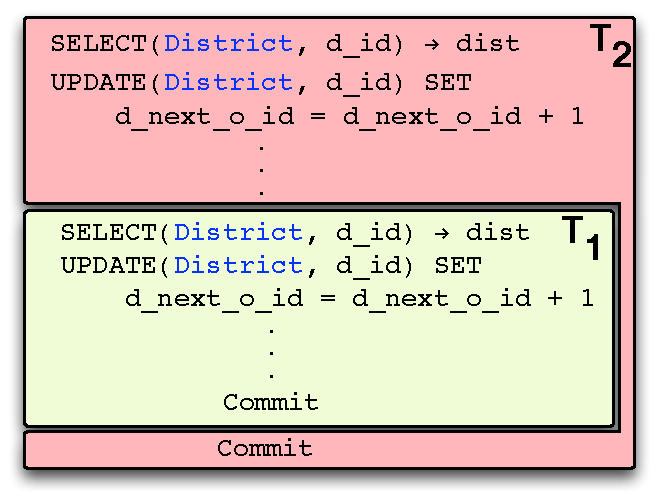
\includegraphics[scale=0.6]{Figures/motiv-eg-1-a}
}
%\hspace*{0.5in}
\subcaptionbox {
  {\sc rc} Execution 2
  \label{fig:motiv-eg-1-b}
}{
  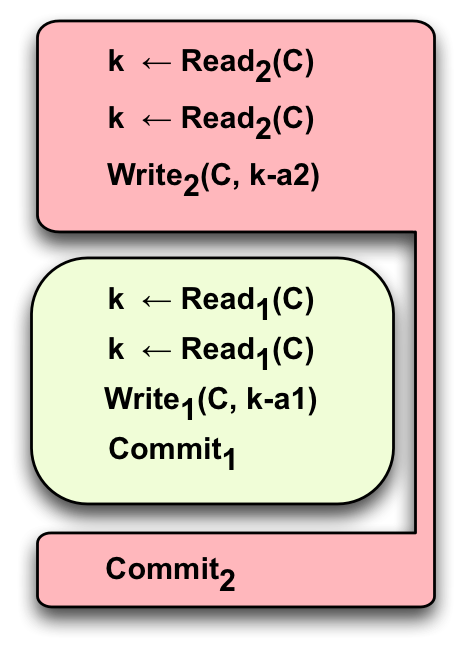
\includegraphics[scale=0.6]{Figures/motiv-eg-1-b}
}
\caption{\small A possible execution of the program shown in Fig.~\ref{fig:motiv-eg-1} under
  \iso{Read Committed} isolation level. Transaction \C{Wd1} is shown
  against lighter green background, and transaction \C{Wd2} against
  darker red background. Each transaction reads the balance (\C{B})
  twice, hence two \C{Reads}.}
\label{fig:rc-ex}
\end{figure}

The figure depicts an execution as a series of read, write, and commit
operations. In the execution on the left, the \C{new\_order} instance
$T_1$ (green) reads the \C{d\_next\_o\_id} field of the district
record for \C{d\_id}, but before it increments the field, another
\C{new\_order} instance ($T_2$) begins its execution and commits. Note
that $T_2$ reads the same \C{d\_next\_o\_id} value as $T_1$, and
inserts new \C{Order} and \C{Order\_line} records with their \C{o\_id}
and \C{ol\_o\_id} fields (resp.) equal to \C{d\_next\_o\_id}. $T_2$
also increments the \C{d\_next\_o\_id} field, which $T_1$ has already
acccessed. This is allowed because reads do not obtain a mutually
exclusive lock on most databases, including PostgreSQL. After $T_2$'s
commit, $T_1$ resumes execution and adds new \C{Order} and
\C{Order\_line} fields with the same order id as $T_1$. Thus, by the
end of the execution, \C{Order\_line} records inserted by $T_1$ and
$T_2$ all bear the same order id. There are also two \C{Order} records
with the same district id (\C{d\_id}) and order id, none of whose
\C{o\_ol\_cnt} reflects the actual number of \C{Order\_line} records
inserted with that order id.  This clearly violates TPC-C's consistency
condition.

Notably, this example does not exhibit any common concurrency bugs
that arise from incorrect use of weak isolation such as
\emph{write-write} conflicts, or \emph{lost updates}.  While $T_1$ and
$T_2$ both increment the \C{d\_next\_o\_id} field of the district
record, they do so atomically (Line 4 of
Fig.~\ref{fig:new_order_code}), allowing both updates to be present in
the final state. Likewise, other well-known anomalies that
characterize RC isolation~\cite{berenson} such as \emph{fuzzy reads},
\emph{phantom reads}, \emph{read skew}, and \emph{write skew}, are
also not exhibited by the example.  Thus, program analyses that aim to
determine appropriate isolation by checking for possible
manifestations of these anomalies would fail to identify grounds for
promoting the isolation level of \C{new\_order} to something stronger.
Yet, if we take the semantics of the application into account, it is
quite clear that RC is not an appropriate isolation level for
\C{new\_order}.

While reasoning in terms of anomalies is cumbersome, and as the above
example shows often inadequate, reasoning about weak isolation in
terms of low-level traces~\cite{adyaphd,gotsmanconcur15} confounds
high-level reasoning and automation.  Another alternative would
interleave weak isolation implementation details within the program,
yielding a (more-or-less) conventional concurrent program that can be
then subject to classical concurrent verification methods.
Considering the size and complexity of real-world transaction systems,
this approach is unlikely to scale.

In this paper, we adopt a different approach that \emph{lifts}
isolation semantics (\emph{not} their implementations) to the
application layer, providing a unified framework to simultaneously
reason about application invariants and isolation properties.  To
illustrate this idea informally, consider how we might verify that
$\C{new_order}$ is sound when executed under a \emph{Repeatable Read}
(RR) isolation level.  PostgreSQL executes an RR transaction by taking
a (conceptual) snapshot of the database state before the transaction
begins that is used by reads performing the transaction.  When the
transaction attempts to update a record, a check is made to determine
if the current version of the record in the database is same as the
snapshot version. If it is, an exclusive lock is obtained on the
record, and the update is performed. If the record is already locked,
the transaction blocks until the lock is released.  When the lock is
obtained, is held exclusively until the transaction commits or rolls
back. If the aforementioned version check fails (i.e., the database
has a later version than the snapshot), the transaction is rolled back
and re-executed.

Although this implementation, comprising many thousands of lines code,
is highly involved, its semantic behavior in terms of how it effects
transitions on the database state is fairly simple.  Since a
transaction's reads are always served from a snapshot, no state
changes are witnessed while the execution is in progress. Thus,
insofar as an RR transaction is concerned, the database state does not
change during the execution.  Uncommitted writes are recorded in a
transaction-local state.  When the transaction commits, the local
state is atomically written to the global state to yield a global
state that reflects the transaction's updates.  However, unlike a
strongly isolated serializable transaction, the commit operation is
performed against the current state of the database, not the
snapshot. Thus, after the transaction finishes execution, but before
it commits, the transaction is able to witness the effects of all
concurrent transactions.  The PostgreSQL RR implementation effectively
constrains this transition.

We can axiomatize this operational description by observing that (a)
due to the version check, the current transaction cannot update a data
item that was already updated by a concurrent transaction, and (b) due
to the use of exclusive write locks, a data item updated by the
current transaction cannot be overwritten by a concurrent transaction.
If $\Delta$ is the state of the database when an RR transactions
finishes, and $\Delta_c$ is the state visible to the transaction at
the point of commit, we know the transition from $\Delta$ to
$\Delta_c$ (written $\Delta \longrightarrow \Delta_c$) cannot exhibit
effects from any concurrent transactions that write to the same data
items as the current RR transaction.  Similarly, if $\delta$ denotes
a local log that relates transaction variables being written with their updated values,
then $\forall x\in\mathit{dom}(\delta)$, $\Delta_c(x) =
\Delta(x)$. To summarize, the operational semantics of PostgresSQL's RR
implementation can be captured as an axiomatization over transitions of
the database state ($\Delta \longrightarrow \Delta'$) during the
lifetime an RR transaction ($T$):
\begin{itemize}
  \item While $T$ executes, $\Delta' = \Delta$.
  \item After $T$ finishes execution, but before it commits its local
    state $\delta$, $\forall(x\in\delta).~\Delta'(x) = \Delta(x)$.
\end{itemize}

This simple characterization of RR isolation allows us to verify the
consistency condtions associated with the \C{new\_order}
transaction. First, since the database doesn't change ($\Delta' =
\Delta$) (where $\Delta'$ represents the state after the transaction
commits), during the execution of the transaction's body, we can
reason about \C{new\_order} as if it executed in complete isolation
until its commit point, leading to a verification process similar to
what would been applied when reasoning about serializability.  When
\C{new\_order} finishes execution and becomes ready to commit, a
transition that transfers the transaction'slocal writes ($\delta$) to
the unchanged database state ($\Delta$).  However, we are required to
consider the interference from concurrent transitions at this point,
which might change the database state from $\Delta$ to $\Delta_c$. If
this interference includes the effects of a concurrent \C{new\_order}
transaction (with the same \C{d\_id}), then verification fails as
described previously (Fig.~\ref{fig:new_order_execs}). Fortunately,
sequential reasoning shows that this is impossible - RR prevents a
concurrent \C{new\_order} transaction that modifies the same
\C{District} record as the current transaction (concretely, since the
record is already present in the current transaction's local log, any
transition from $\Delta$ to $\Delta_c$ cannot change this record).
Applying such axiomatic reasoning on \C{new\_order} allows us to prove
that the TPC-C invariant holds when the transaction is executed under
PostgreSQL's RR isolation.  Our proof framework generalizes this style
of reasoning to various isolation levels on databases.

The second observation that informs our approach is one that pertains
to automation. Program verification, even when machine-aided, often
entails significant annotation burden in the form of intermediary
assertions and loop invariants required to prove a program correct.
This is certainly true for concurrent program logics, such as
Rely-Gurantee, which extend Hoare logic with additional artifacts and
where (stable) intermediary assertions and loop invariants remain a
major source of annotation burden.  However, a relational database is
a significantly simpler abstraction than shared memory. There are no
pointers, or linked data structures, or aliasing.  Although a database
essentially abstracts a mutable state, the state is mutated through a
well-defined fixed number of interfaces (SQL statements), each tagged
with a logical formula describing what records are accessed and
updated. 

This observation leads us away from thinking of database transactions
as concurrent imperative programs.  Instead, we see value in viewing
them as essentially functional computations that manage database state
monadically~\cite{statemonad}. We find it useful to reason about
statements that mutate the database state, not in terms of a pre- and
post-condition pair, but in terms of a state transformer that relates
the pre- and post-states of a statement. This state transformer
semantics can be defined algorithmically, just like predicate
transformer semantics (e.g., strongest post-condition).  Here, a state
transformer interprets a SQL statement in the set domain, taking
advantage of the fact that a a database is essentially a set of
tuples, and a SQL statement is a transformer over these sets.  The
benefit of this approach is that low-level loops can now be
substituted with higher-order combinators that automatically lift the
state transformer of its higher-order argument (i.e., the loop body)
to the state transformer of the combined expression (i.e., the loop).
Thus the semantics of a \C{foreach} loop, for instance, can be
captured as a state transformer, where the state is a set, and the
transformation defines a bind operation. We illustrate this intuition
on a simple example.

% \begin{figure}[!t]
% \centering
% %
% \begin{subfigure}[b]{0.46\textwidth}
% \begin{ocaml}
% Set s' = $\emptyset$;
% foreach x in s {
%   s'.add(f(x)); 
% }
% \end{ocaml}
% \caption{}
% \end{subfigure}
% %
% \begin{subfigure}[b]{0.5\textwidth}
% \begin{ocaml}
% let s' = ref [];
% foreach s (fun x -> s' := x::(!s'));
% \end{ocaml}
% \caption{Lorem ipsum, lorem ipsum,Lorem ipsum, lorem ipsum,Lorem ipsum}
% \end{subfigure}
% \caption{Caption place holder}
% %
% \caption{New versions are created from existing versions either
% through \C{push} or \C{merge}.}
% \label{fig:syntactic-ancestors}
% \end{figure}
% let s' = ref (Set.empty) in
% foreach xs @@ fun x -> 
%   begin
%     s' := Set.union !s' @@ 
%             Set.map_selected s (fun y -> y<x)
%                                (fun y -> y+x);
%     s' := Set.add !s' x;
%   end
\begin{figure}[!h]
\begin{ocaml}
foreach item_reqs @@ fun item_req -> do
  SQL.update Stock (fun s -> {s with s_qty = k1}) 
                   (fun s -> s.s_i_id = item_req.ol_i_id);
  SQL.insert Order_line {ol_o_id=k2; ol_d_id=k3; 
                         ol_i_id=item_req.ol_i_id; ol_qty=item_req.ol_qty}
\end{ocaml}
\caption{Foreach loop from Fig.~\ref{fig:new_order_code}}
\label{fig:foreach_code}
\end{figure}

Fig.~\ref{fig:foreach_code} shows a (simplified) snippet of code taken
from Fig.~\ref{fig:new_order_code}. Some irrelevant expressions have
been replaced with constants (\C{k1} to \C{k3}).  The body of the loop
executes a SQL update followed by an insert.  Recall that a transaction
reads from the global database ($\Delta$), and writes to a
transaction-local database ($\delta$) before committing these updates. An update
statement filters the tuples that match the search criteria from $\Delta$
and computes the updated tuples that are to be
added to the local database. Thus, its state transformer (call it
$T_U$) is the following function on sets\footnote{$\bind$ has higher precedence than $\cup$.}:
\begin{ocaml}
  fun ($\Delta$,$\delta$) -> $\delta$ $\cup$ $\Delta$$\bind$(fun s -> if table(s) = stock && s.s_i_id = item_req.ol_i_id 
                                 then {{s with s_qty = k1}} (* a singleton set *)
                                 else $\emptyset$)
\end{ocaml}
% \begin{smathpar}
% \begin{array}{c}
%   \lambda\Delta.\lambda\delta.\, \delta \;\cup\; 
%       \Delta \,\bind\, (\lambda s.\, 
%           \C{if}\;{\C{stock}(s) \conj 
%                    \C{s.s\_i\_id} = \C{item\_req.ol\_i\_id}}\\
%            \hspace*{0.9in}
%            \C{then}\;{\{\{s \;\C{with}\; \C{s\_qty} = \C{k1}\}\}}\;
%            \C{else}\;{\emptyset})
% \end{array}
% \end{smathpar}
% \begin{verbatim}
%   Rmem(σ'(s')) = Rmem(σ(s')) U 
%                  Rmem[\x. Rmem[\y. if y<x then {y+x} else {}](σ(s)) U {x}](xs)
% \end{verbatim}
Observe that
$T_U(\Delta,\delta)$ is of the form $\delta \,\cup\,
F_U(\Delta)$. The transformer ($T_I(\Delta,\delta)$)
for the subsequent \C{insert} statement can be similarly calculated to
be of the form $\delta \cup F_I(\Delta)$.
Their composition gives the state transformer of the loop body:
\begin{ocaml}
  fun ($\Delta$,$\delta$) -> $\delta$ $\cup$ $F_U(\Delta) \,\cup\, F_I(\Delta)$
\end{ocaml}
Let $F_{body}(\Delta) = F_U(\Delta) \,\cup\, F_I(\Delta)$.   The
transformer for the \C{foreach} loop can now be computed as following:
\begin{ocaml}
  fun ($\Delta$,$\delta$) -> $\delta$ $\cup$ item_reqs$\bind$(fun item_req -> $F_{body}(\Delta)$)
\end{ocaml}
Observe that the transformer captures the precise semantics of the
loop as a formula in the domain of sets extended with a bind
function. The advantage in doing so is that we can now make use of a
semantics-preserving translation from this domain to first-order
logic, allowing us to leverage SMT solvers for automatic proofs
without having to infer loop invariant, or provide intermediate
assertions.  Sec.~\ref{sec:automation} describes this translation. In
the exposition thus far, we assumed $\Delta$ remains invaraint, which
is clearly not the case when we admit concurrency.  Necessary
concurrency extensions of the state transformer semantics is also
covered in Sec.~\ref{sec:automation}.  The immediate two sections,
however, focus on laying theoretical foundations for reasoning about
weak isolation.
